
%=======================

%Магомедов М.А.
\section{Исследование модели Поттса на треугольной решетке алгоритмом Ванга-Ландау}



%\section{Аннотация}
%
%Модель Поттса на треугольной решетке с учетом взаимодействия как первых, так и вторых ближайших соседей, исследована алгоритмом Ванга -- Ландау метода Монте-Карло. Вычислена плотность состояний системы и рассчитаны температурные зависимости энтропии $S$. Показано, что в зависимости от соотношений обменных взаимодействий между первыми и вторыми ближайшими соседями, основное состояние может быть как сильно вырожденным, что свидетельствует о наличии фрустрации в системе, так и слабо вырожденным.
%
%Определены структуры основного состояния и показано, что в данной системе реализуется Страйповое, триплетное или смешанное страйпово-триплетное состояние для фазы $1$, неупорядоченное сильно вырожденное состояние или многослойное слабо вырожденное состояние для фрустрированной фазы и упорядоченное ферромагнитное состояние для ферромагнитной фазы.
%
%Показано, что фазовый переход из ферромагнитной и страйповой-триплетной фаз в парамагнитную является фазовым переходом первого рода, в то время как переход из фрустрированной области в парамагнитную является переходом второго рода. Рассчитаны температурные зависимости различных термодинамических параметров. Определены температуры фазовых переходов и построена фазовая диаграмма системы.




\subsection{Предварительные сведения}


В последние годы  значительное внимание уделяется экспериментальному и теоретическому исследованию различных низкоразмерных, квазиодномерных или двумерных систем, в том числе наноструктур. Такие системы обладают рядом интересных свойств, перспективных в плане практического применения в различных электронных устройствах. Изучение различных свойств этих объектов открывает широкие перспективы для экспериментальных приложений. В ближайшие годы нанотехнологии позволят совершить поистине гигантский технологический скачок в самых различных областях науки и техники \cite{ph3_1}.

Одними из таких материалов являются делафосситы, названные в честь французского кристаллографа XIX века Ж. Делафосса  (Delafosse) \cite{ph3_2, ph3_3}. Делафосситы имеют общую химическую формулу $A+B3+X2$, где $А$ и $В$ -- катионы, $Х$ -- кислород. Одним из ярких представителей семейства делафосситов, является $CuFeO_2$, структура которого приведена на рисунке \ref{phys3-pic-47}.

\begin{figure}[H]
	\centering
	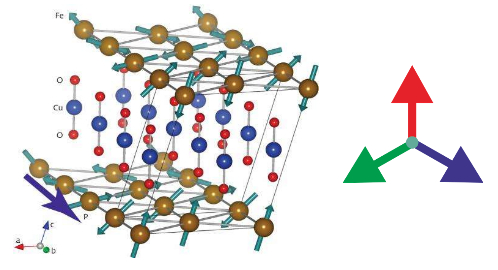
\includegraphics[width=0.5\linewidth]{content/sections/images/phys3-1}
	\caption{Структура делафоссита $CuFeO_2$. Справа приведено схематическое и цветовое изображение трех возможных направлений ориентации спинов в трехвершинной  модели Поттса}\label{phys3-pic-47}
\end{figure}





Таким образом, $CuFeO_2$ имеет явно выраженную плоскостную структуру, взаимодействием между слоями можно пренебречь.

Схематическое и цветовое изображение трех возможных направлений ориентации спинов  Fe  в материале $CuFeO_2$  приведено на вставке рисунке \ref{phys3-pic-47}. Таким образом, имеется три возможных направления спинов железа. Данная система хорошо описывается моделью Поттса с числом состояний $q = 3$.

Гамильтониан модели Поттса с числом состояний $q = 3$ может быть представлен в следующем виде \cite{ph3_4}:
\begin{equation}
	H = -J_1 \sum_{i,j}\cos\theta_{i,j}-J_2\sum_{i,k}\cos\theta_{i, k}
\end{equation}
где $J_1$ и $J_2$ -- параметры обменного взаимодействия для ближайших и вторых ближайших соседей. $\theta_{i,j}$, $\theta_{i,k}$ -- углы между взаимодействующими спинами $S_i - S_j$ и $S_i - S_k$ соответственно.

Численные расчеты, проведенные в работе \cite{ph3_4}, показали, что при учете только первых ближайших соседей с величиной $J_1<0$, эта модель демонстрирует поведение характерное для ФП первого рода. При учете первых и вторых ближайших соседей с величинами $J_1<0$ и $J_2<0$ соответственно в рассматриваемой модели возможны фрустрации. На данном этапе исследований нами проведены исследования модели Поттса при $J_1 = 0$ и различных значениях $J_2$.




\subsection{Структура основного состояния и фазовая диаграмма трехвершинной модели Поттса на треугольной решетке}

Далее нами приводятся результаты исследования модели Поттса на треугольной решетке методом Ванга -- Ландау \cite{ph3_4, ph3_5, ph3_6, ph3_7}.
На рисунке \ref{phys3-pic-20} приведена зависимость энергии основного состояния от величины второго обменного взаимодействия $J_2$. Как наглядно видно из рисунка, в системе реализуются один из трех вариантов упорядочения спинов, энергия которых приведены разными цветами. В зависимости от величины $J_2$ приоритетным оказывается один из этих сценариев.

\begin{figure}[H]
	\centering
	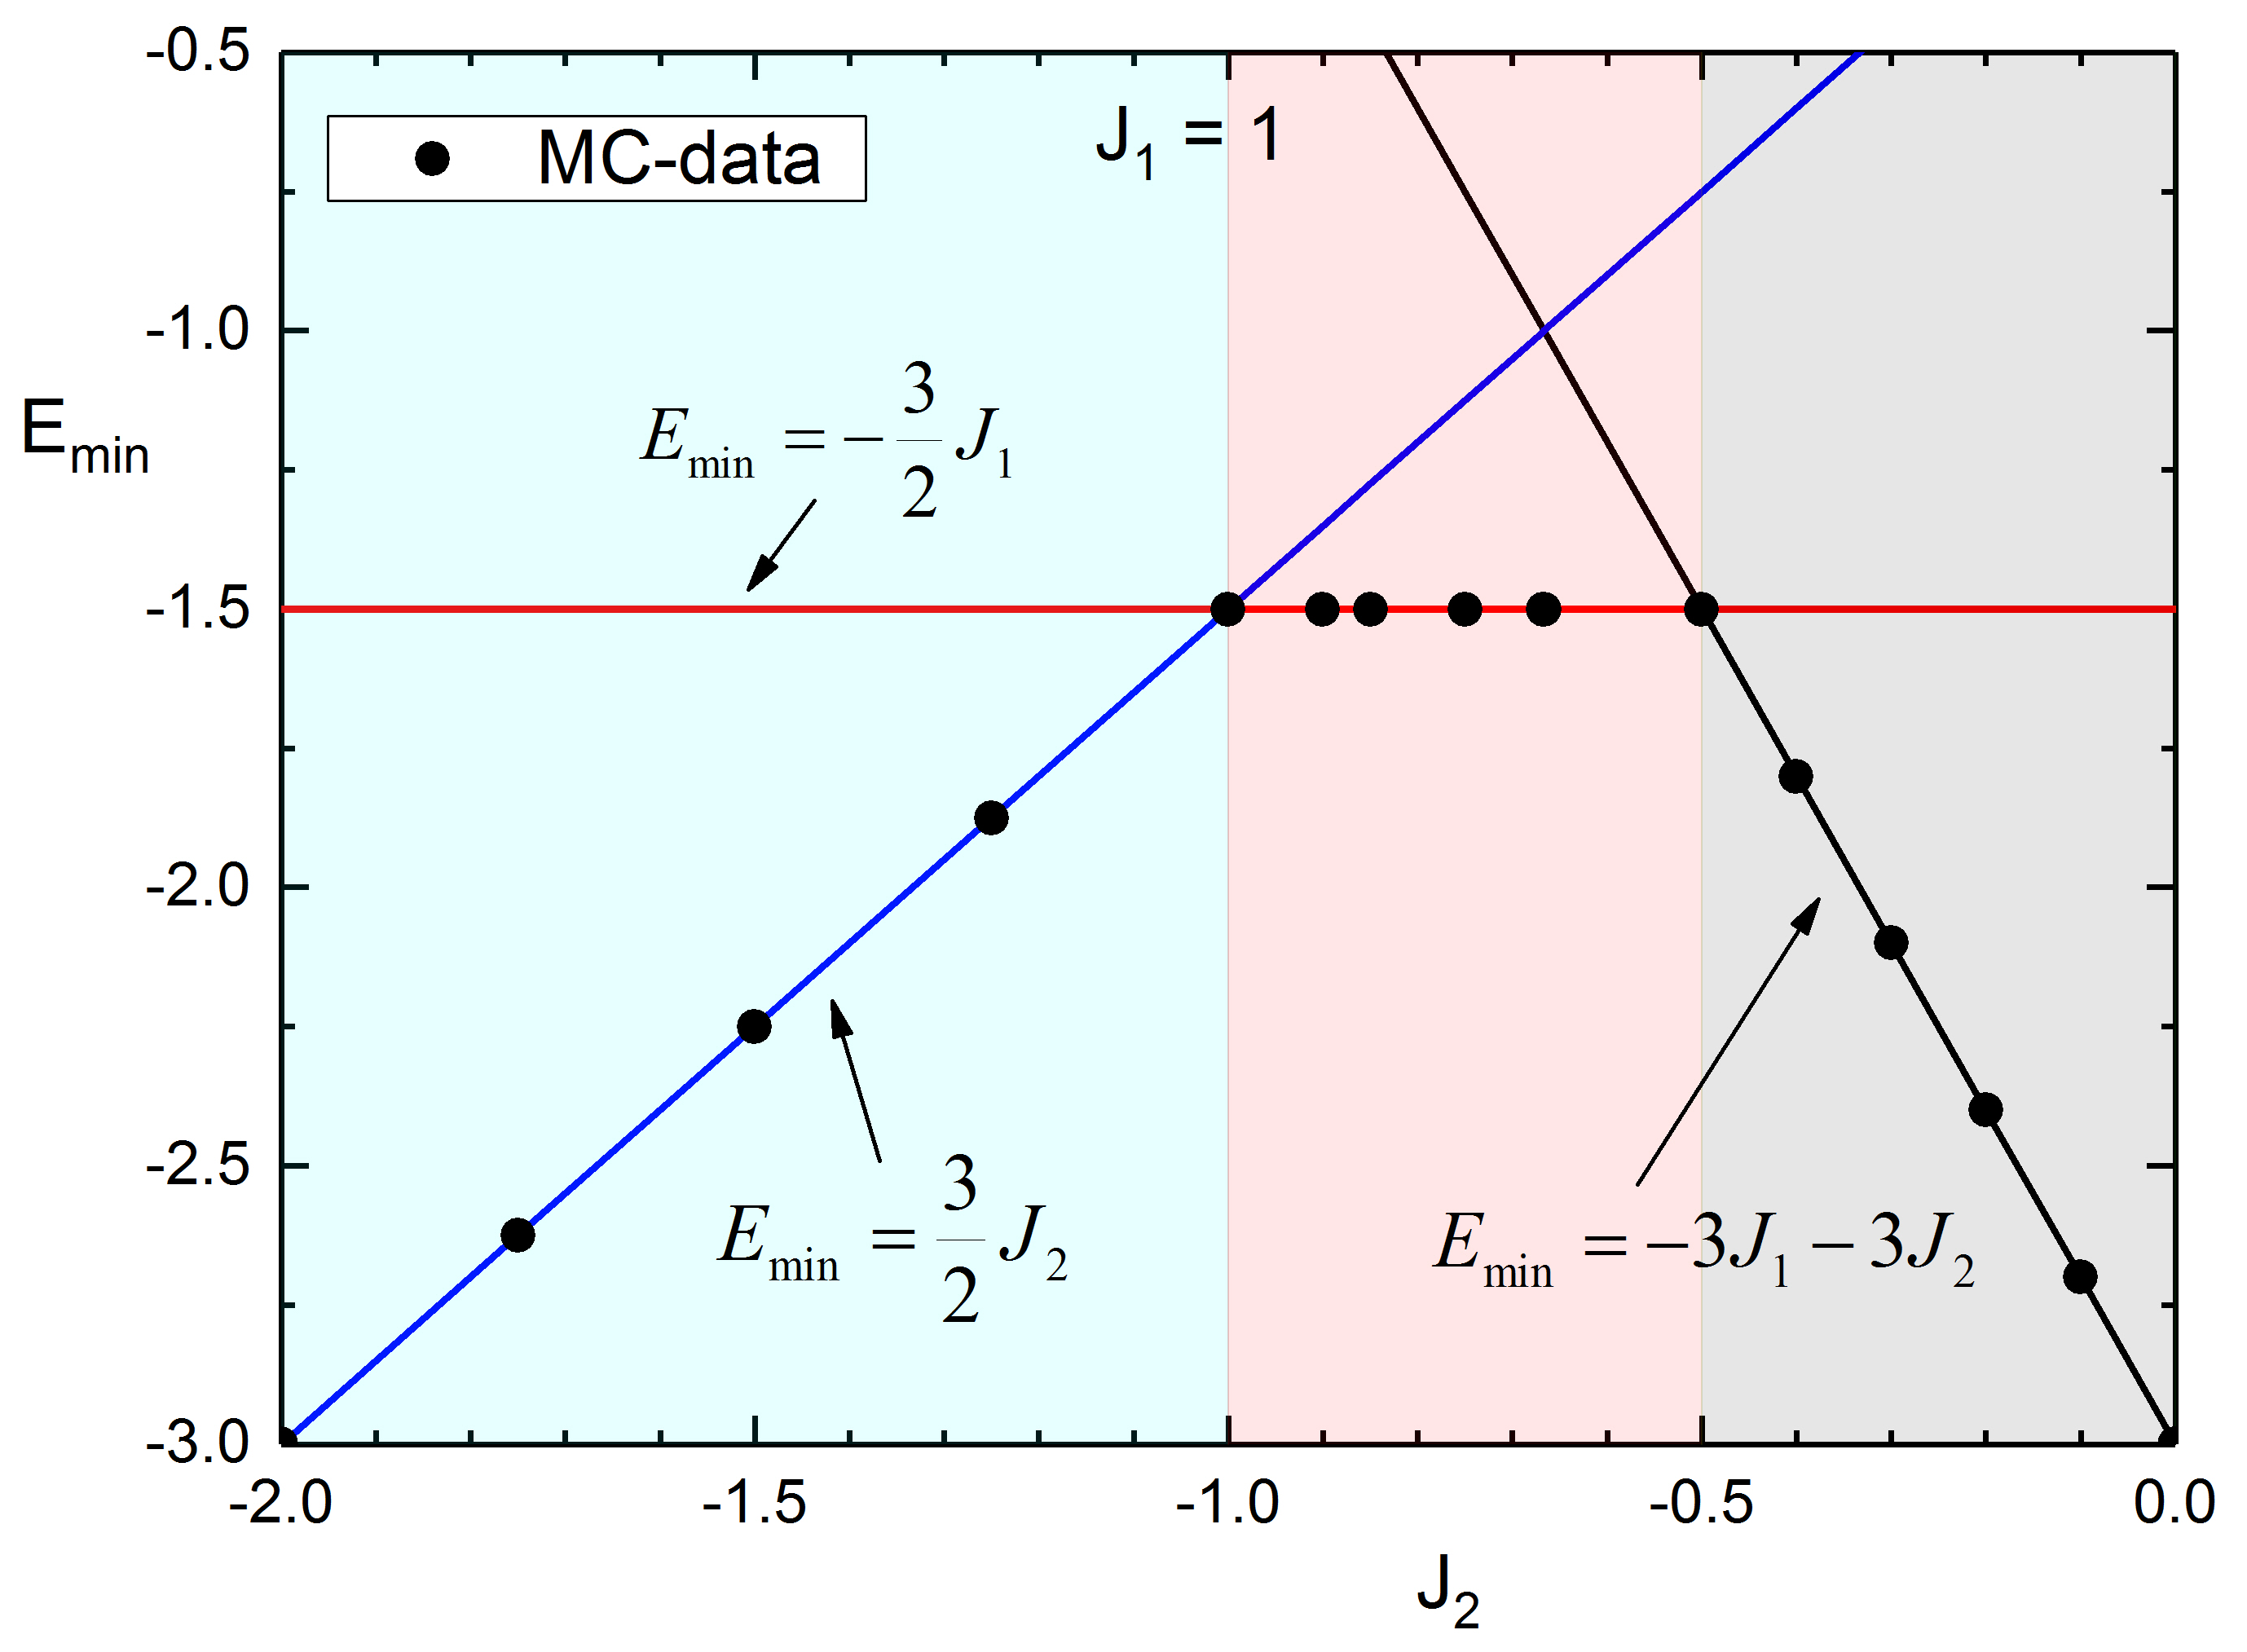
\includegraphics[width=0.5\linewidth]{content/sections/images/phys3-2}
	\caption{Зависимость энергии основного состояния от величины второго обменного взаимодействия $J_2$}
\label{phys3-pic-20}
\end{figure}

На рисунке \ref{phys3-pic-30} приведена зависимость плотности состояний, рассчитанная методом Ванга -- Ландау, от величины второго обменного взаимодействия $J_2$. Плотность состояний имеет куполообразную форму с максимумом при нуле. При некоторых значениях $J_2$ основное состояние вырождено.

\begin{figure}[H]
	\centering
	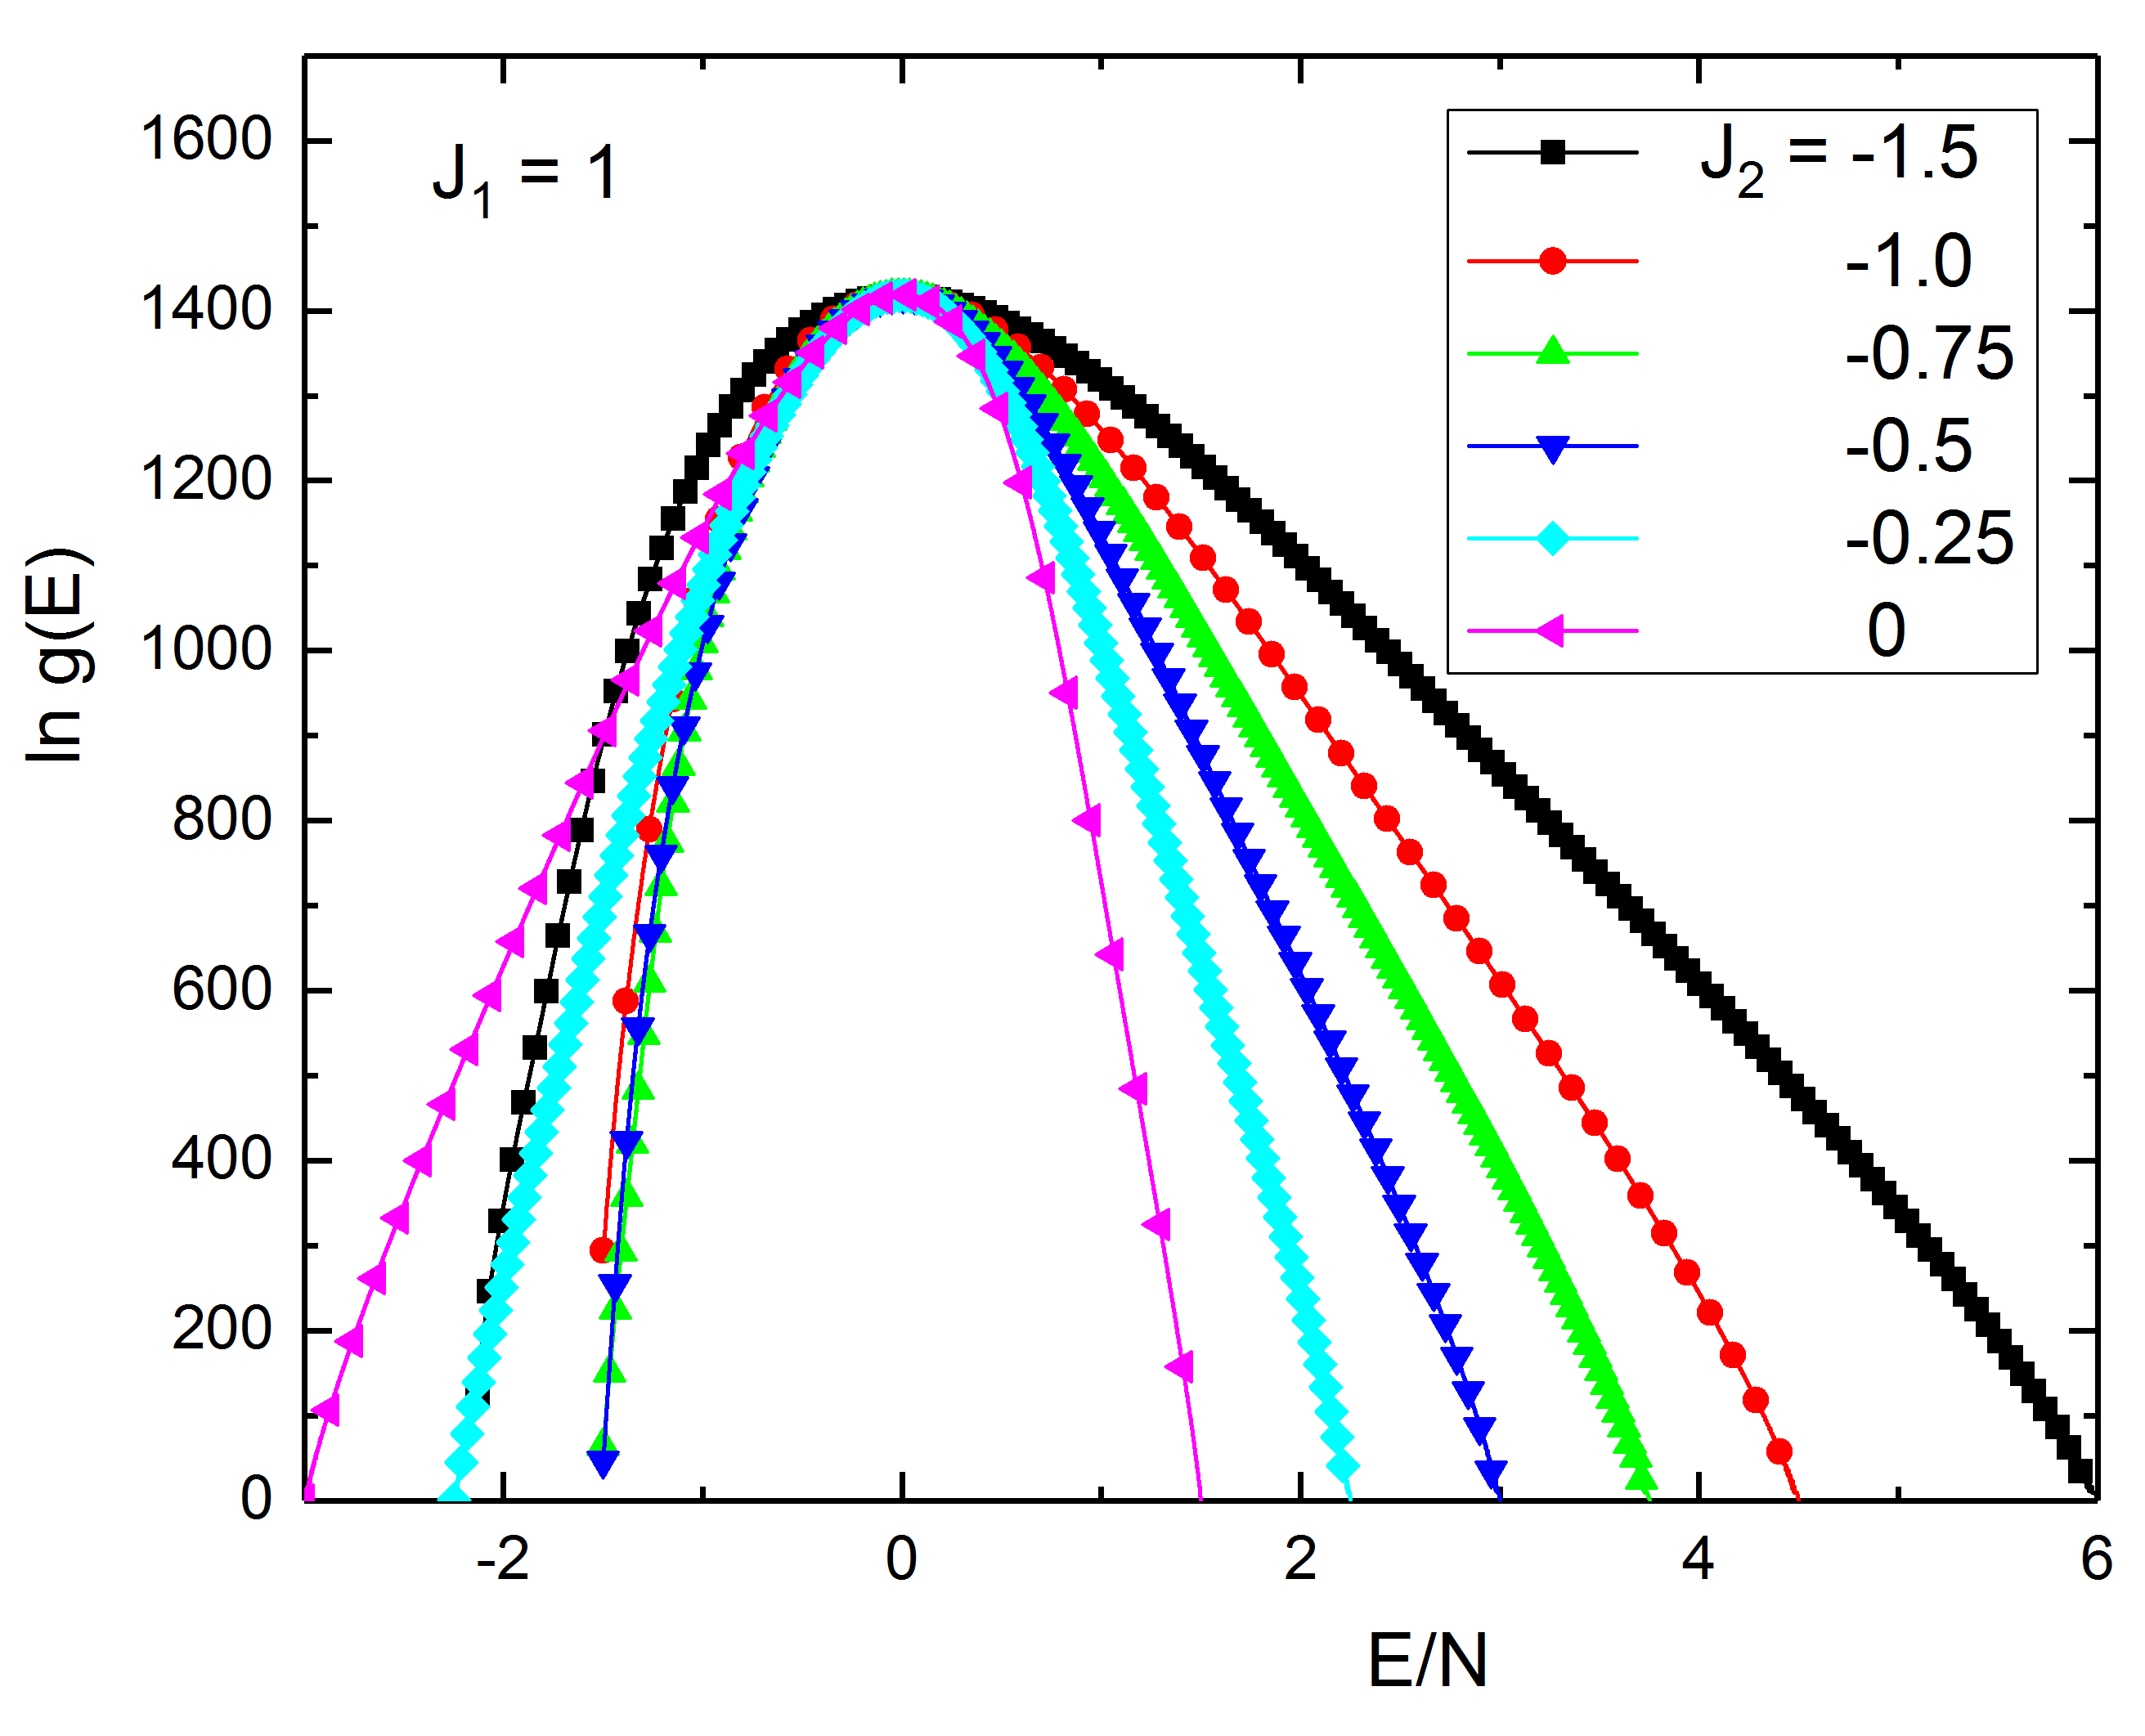
\includegraphics[width=0.5\linewidth]{content/sections/images/phys3-3}
	\caption{Зависимость плотности состояний от величины второго обменного взаимодействия $J_2$}
\label{phys3-pic-30}
\end{figure}

Для определения температуры фазового перехода и его типа использовался метод производной от плотности состояний \cite{ph3_7}. Пример определения точки фазового перехода данным методом приведен на рисунке \ref{phys3-pic-40}.

\begin{figure}[H]
	\centering
	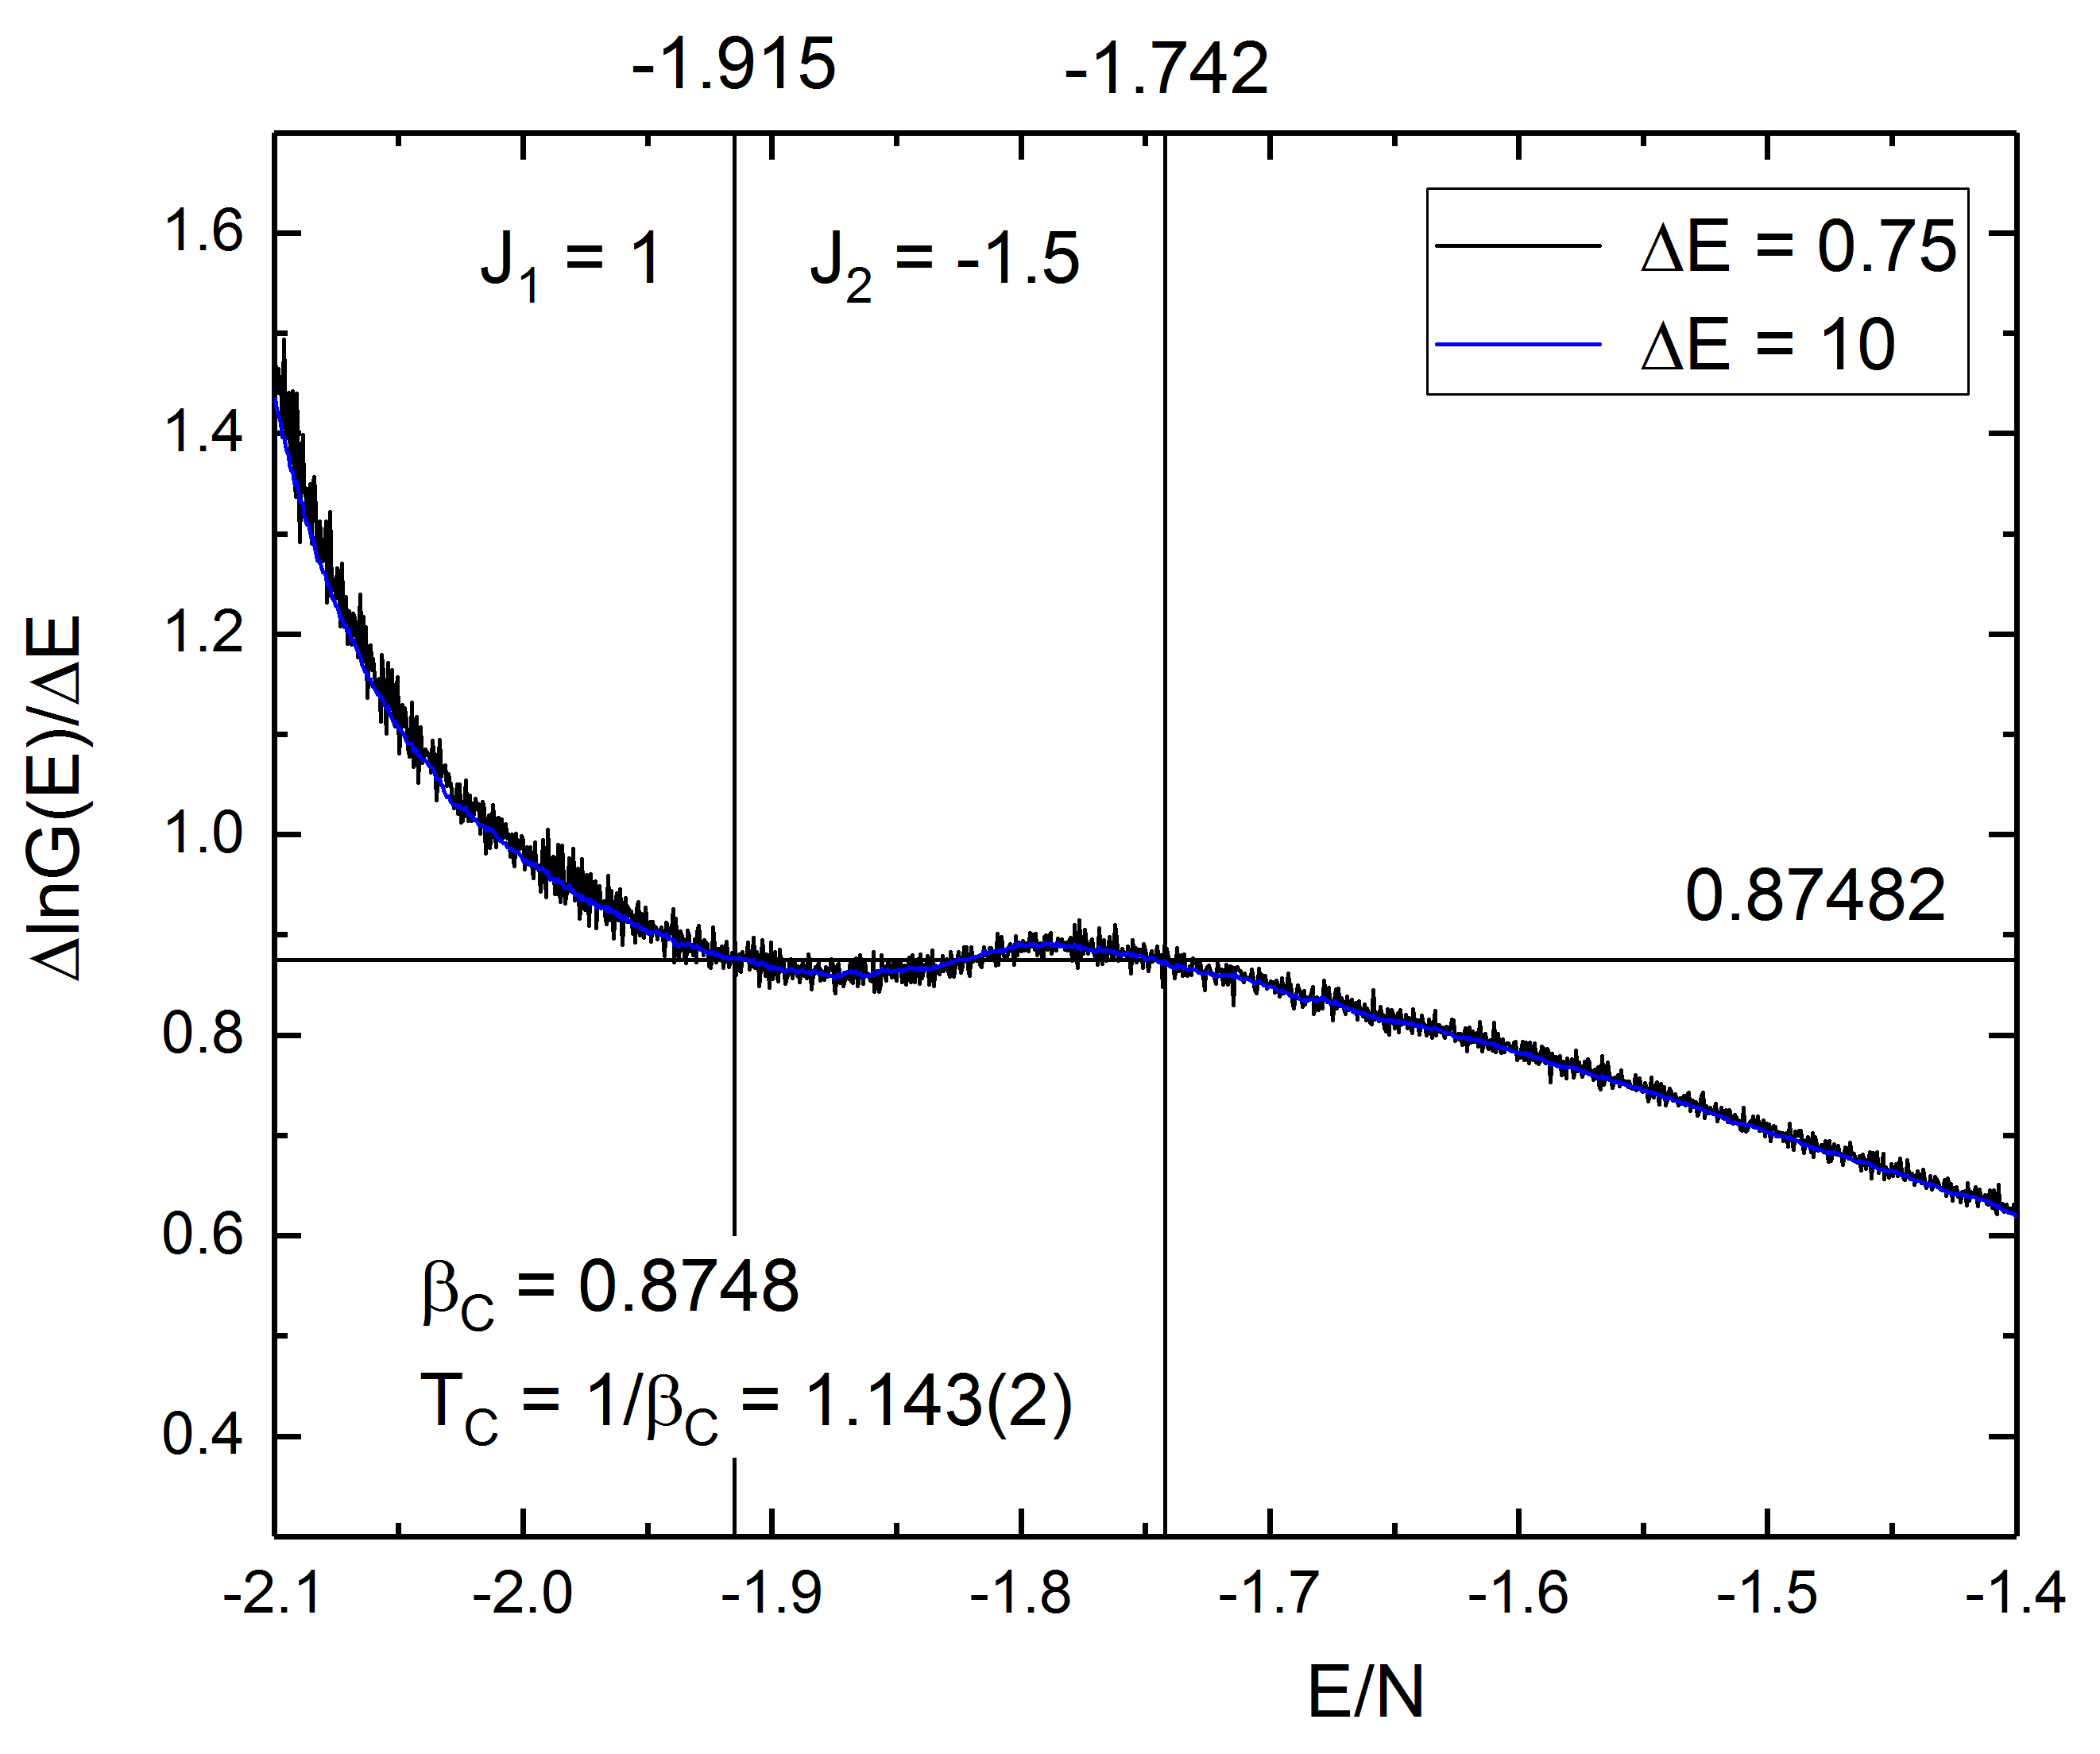
\includegraphics[width=0.5\linewidth]{content/sections/images/phys3-4}
	\caption{Производная от плотности состояний при $J_1 = 1$ и $J_2 = -1.5$}
\label{phys3-pic-40}
\end{figure}

Зная плотность состояний системы можно рассчитать температурную зависимость любого интересующего нас термодинамического параметра. На рисунке \ref{phys3-pic-50} приведена температурная зависимость энтропии системы, рассчитанная из плотности состояний, при различных значениях обменного взаимодействия. Как видно из рисунка, при высоких температурах энтропия стремится к теоретическому значению $\ln{3}$. С понижением температуры в зависимости от величины $J_2$ энтропия может как обнуляться, так и стремиться к некоторому ненулевому значению.

\begin{figure}[H]
	\centering
	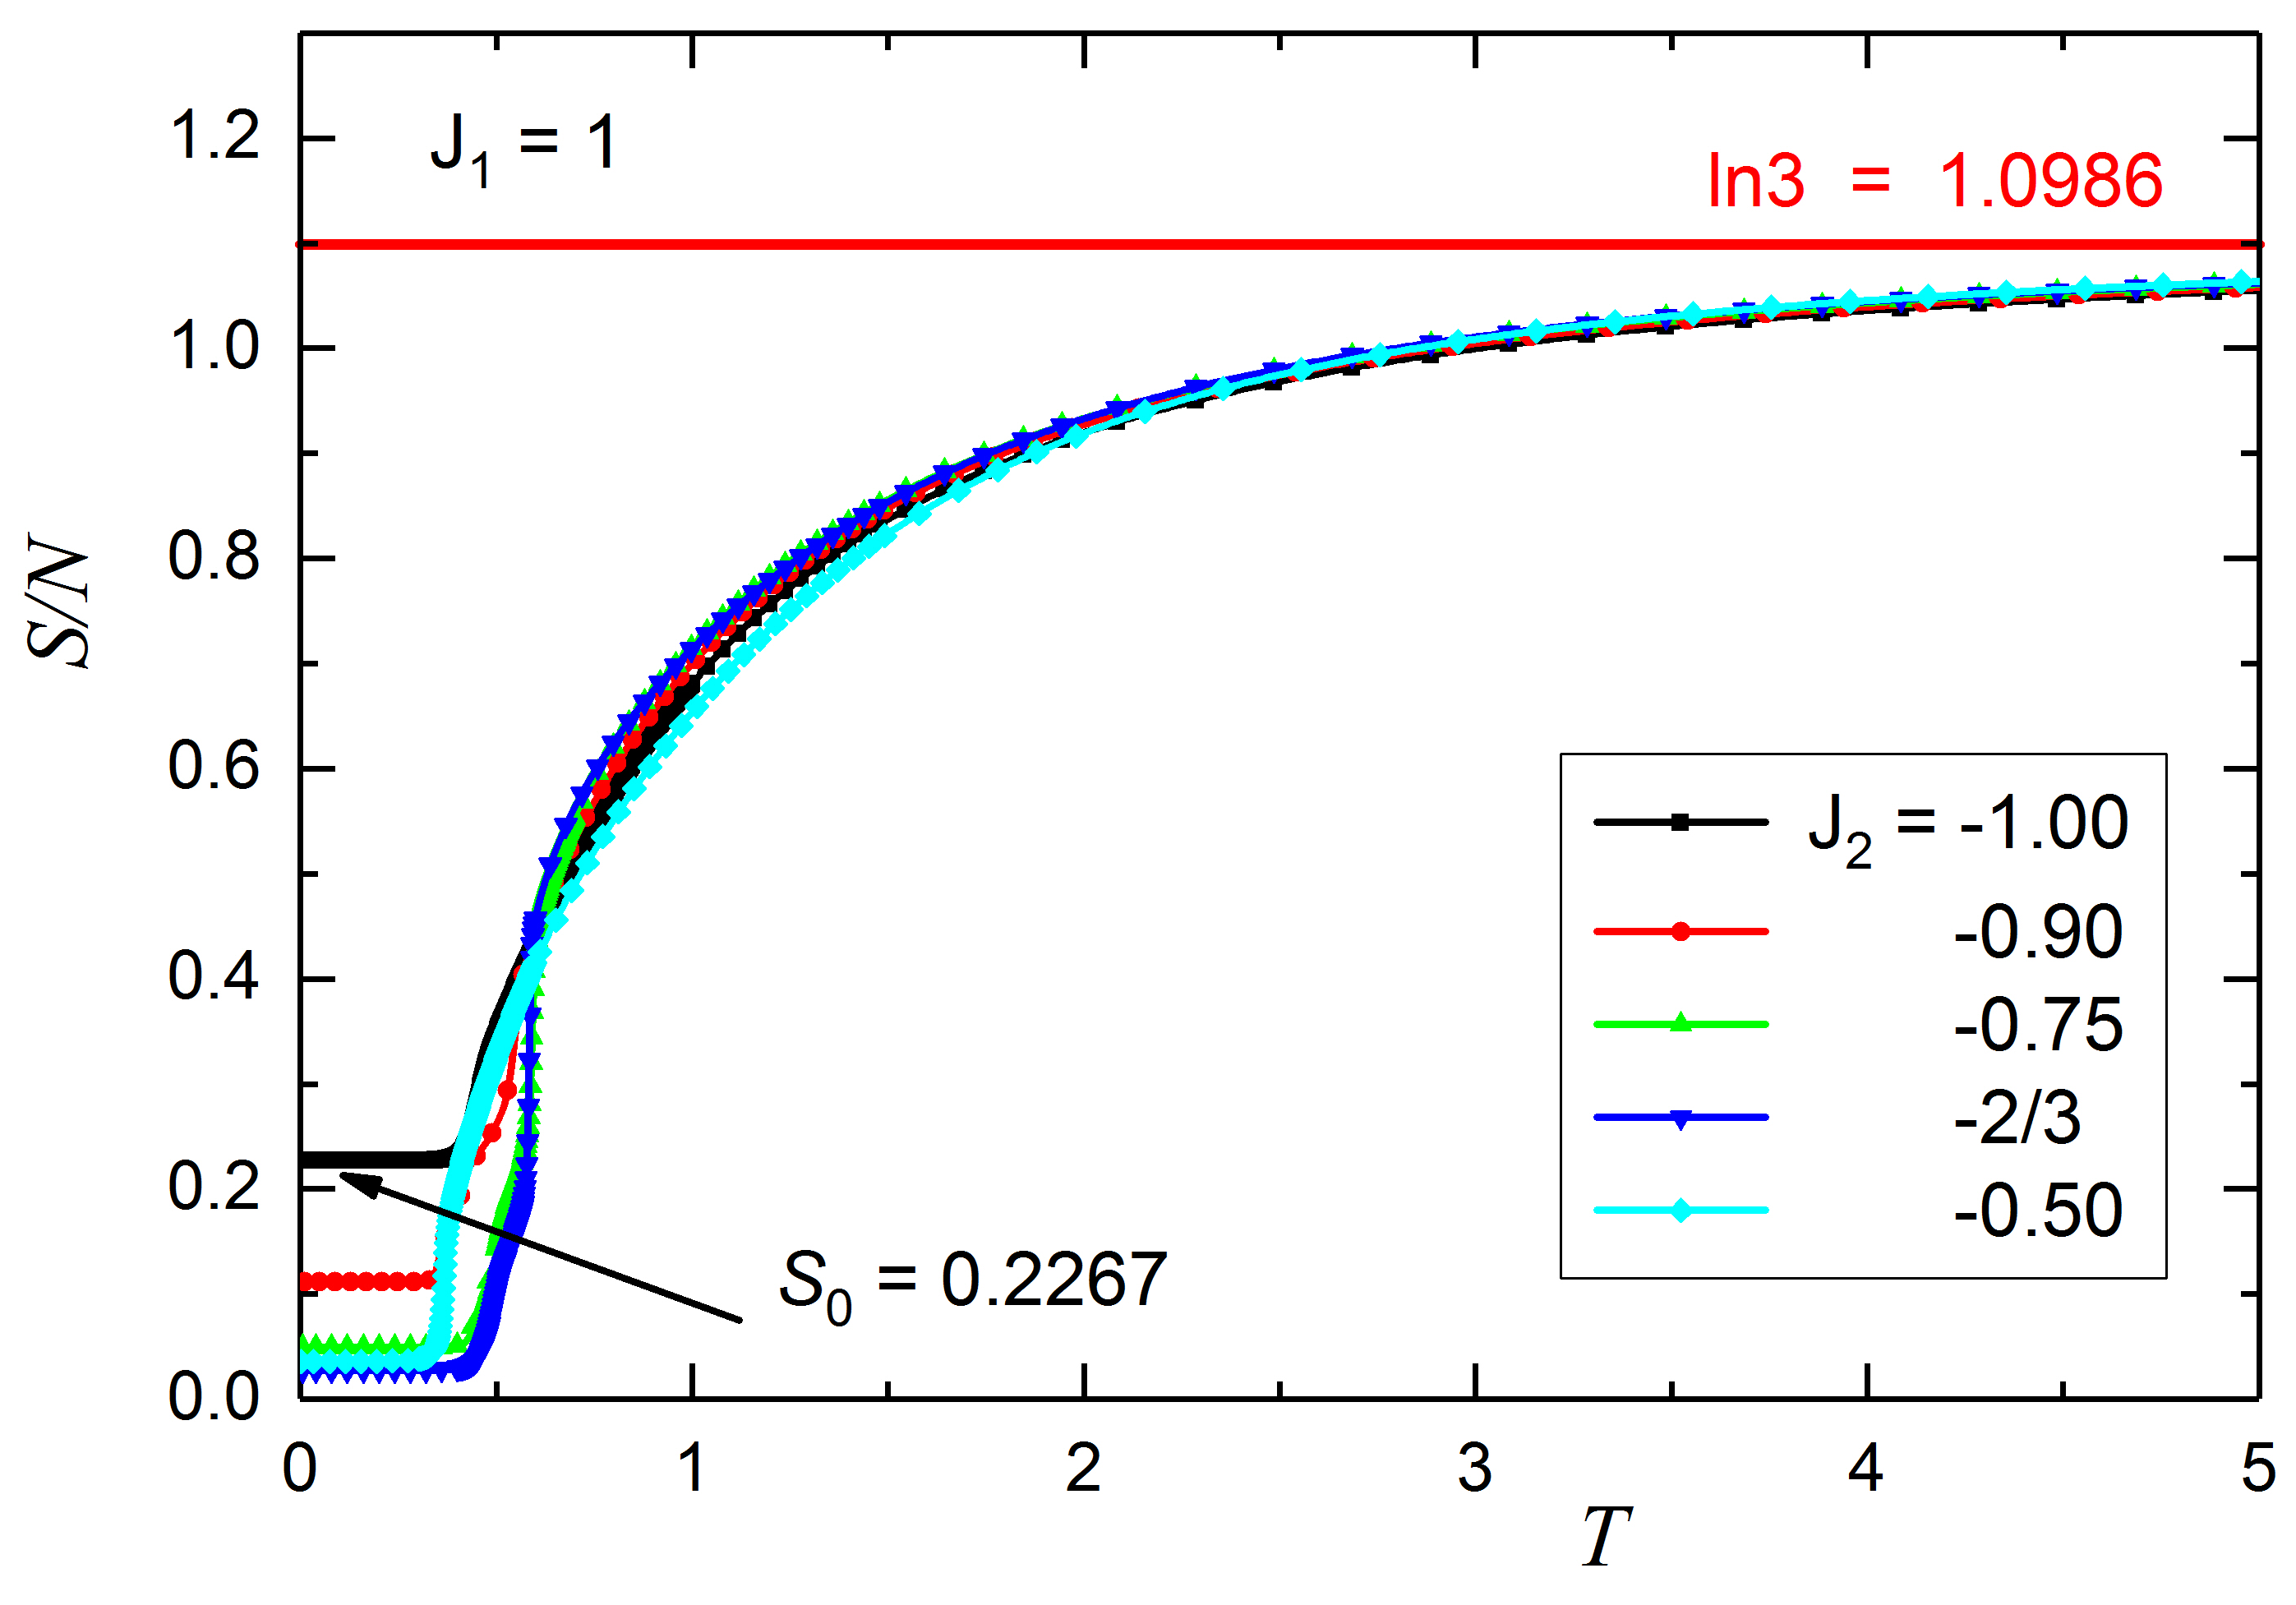
\includegraphics[width=0.5\linewidth]{content/sections/images/phys3-5}
	\caption{Температурная зависимость энтропии системы при $J_1 = 1$ и различных $J_2$}
\label{phys3-pic-50}
\end{figure}

В результате анализа основного состояния системы были определены структуры основного состояния, приведенные на рисунке \ref{phys3-pic-60}.

\begin{figure}[H]
	\centering
	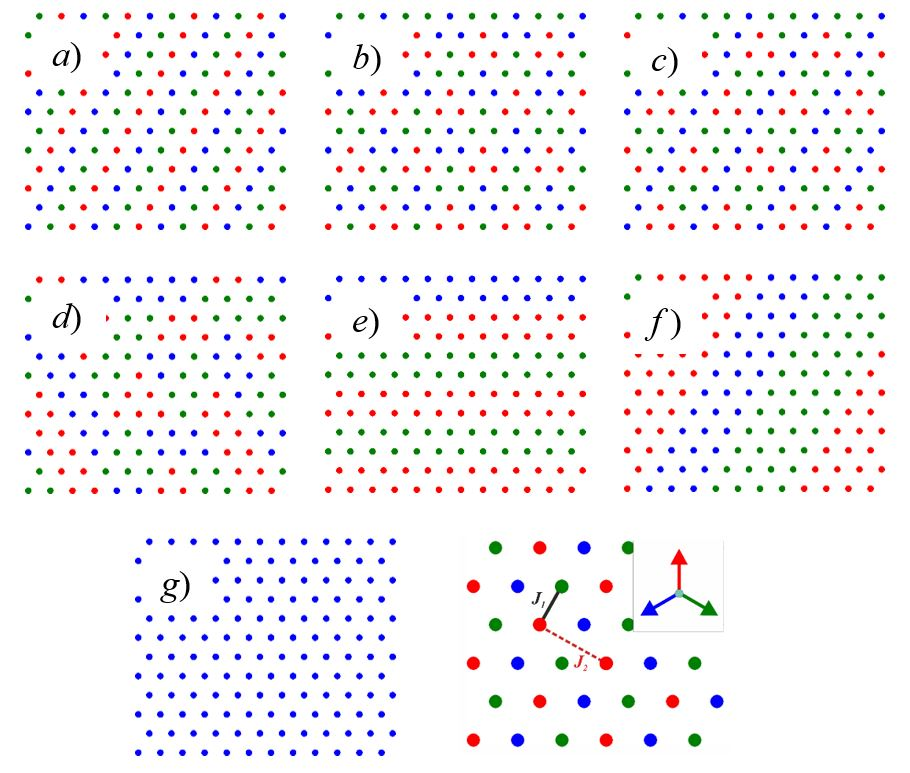
\includegraphics[width=0.5\linewidth]{content/sections/images/phys3-6}
	\caption{Структуры основного состояния, реализуемые в системе при $J_1 = 1$ и различных значениях $J_2$}
\label{phys3-pic-60}
\end{figure}

Фазовая диаграмма системы приведена на рисунке \ref{phys3-pic-70}. На рисунке также в фигурных скобках приведены соответствующие данной фазе структуры с рисунка \ref{phys3-pic-60}.

\begin{figure}[H]	
	\centering
	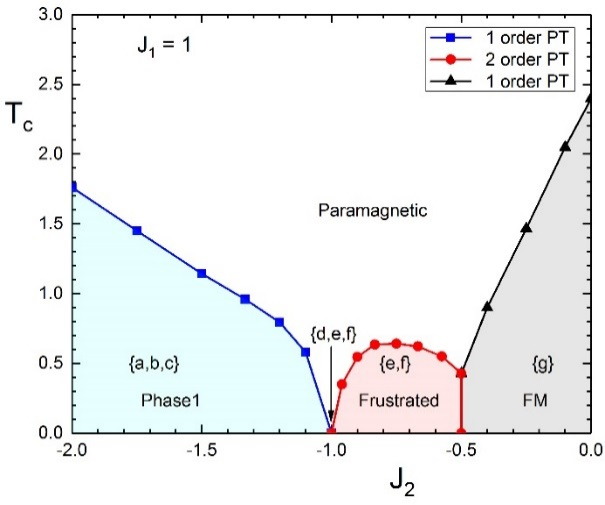
\includegraphics[width=0.5\linewidth]{content/sections/images/phys3-7}
	\caption{Фазовая диаграмма модели Поттса}
\label{phys3-pic-70}
\end{figure}

Как видно из рисунка, в зависимости от величин обменных взаимодействий, с понижением температуры системе возможны три сценария упорядочения:

\begin{itemize}
	\item
	Страйповое (рисунок \ref{phys3-pic-60}.а), триплетное (рисунок \ref{phys3-pic-60}.b) или смешанное \linebreak страйпово-триплетное состояние (рисунок \ref{phys3-pic-60}.c);
	
	\item
	Фрустрированное неупорядоченное(рисунок \ref{phys3-pic-60}.d) или многослойное состояние (рисунок \ref{phys3-pic-60}.e, \ref{phys3-pic-60}.f);
	
	\item
	Упорядоченое ферромагнитное состояние (рисунок \ref{phys3-pic-60}.g).
\end{itemize}

%\section{Заключение}
%
%Методом Ванга -- Ландау исследована модель Поттса с числом состояний $q=3$ на треугольной решетке с учетом обменного взаимодействия между первыми и вторыми ближайшими соседями. Вычислена плотность состояний системы и рассчитаны температурные зависимости энтропии $S$. Показано, что в зависимости от соотношений обменных взаимодействий между первыми и вторыми ближайшими соседями, основное состояние системы может быть сильно вырожденным.
%
%Определены структуры основного состояния и показано, что в данной системе реализуется Страйповое, триплетное или смешанное страйпово-триплетное состояние для фазы $1$, неупорядоченное сильно вырожденное состояние или многослойное слабо вырожденное состояние для фрустрированной фазы и упорядоченное ферромагнитное состояние для ферромагнитной фазы.
%
%Показано, что фазовый переход из ферромагнитной и страйповой-триплетной фаз в парамагнитную является фазовым переходом первого рода, в то время как переход из фрустрированной области в парамагнитную является переходом второго рода. Определены температуры фазовых переходов и построена фазовая диаграмма системы.





